\newcommand{\rAnt}{R_\text{a}}
% mnras_template.tex
%
% LaTeX template for creating an MNRAS paper
%
% v3.0 released 14 May 2015
% (version numbers match those of mnras.cls)
%
% Copyright (C) Royal Astronomical Society 2015
% Authors:
% Keith T. Smith (Royal Astronomical Society)

% Change log
%
% v3.0 May 2015
%    Renamed to match the new package name
%    Version number matches mnras.cls
%    A few minor tweaks to wording
% v1.0 September 2013
%    Beta testing only - never publicly released
%    First version: a simple (ish) template for creating an MNRAS paper

%%%%%%%%%%%%%%%%%%%%%%%%%%%%%%%%%%%%%%%%%%%%%%%%%%
% Basic setup. Most papers should leave these options alone.
\documentclass[a4paper,fleqn,usenatbib]{mnras}

% MNRAS is set in Times font. If you don't have this installed (most LaTeX
% installations will be fine) or prefer the old Computer Modern fonts, comment
% out the following line
\usepackage{newtxtext,newtxmath}
% Depending on your LaTeX fonts installation, you might get better results with one of these:
%\usepackage{mathptmx}
%\usepackage{txfonts}

% Use vector fonts, so it zooms properly in on-screen viewing software
% Don't change these lines unless you know what you are doing
\usepackage[T1]{fontenc}
\usepackage{ae,aecompl}


%%%%% AUTHORS - PLACE YOUR OWN PACKAGES HERE %%%%%

% Only include extra packages if you really need them. Common packages are:
\usepackage{graphicx}	% Including figure files
\usepackage{amsmath}	% Advanced maths commands
\usepackage{amssymb}	% Extra maths symbols

%%%%%%%%%%%%%%%%%%%%%%%%%%%%%%%%%%%%%%%%%%%%%%%%%%

%%%%% AUTHORS - PLACE YOUR OWN COMMANDS HERE %%%%%

% Please keep new commands to a minimum, and use \newcommand not \def to avoid
% overwriting existing commands. Example:
%\newcommand{\pcm}{\,cm$^{-2}$}	% per cm-squared

%%%%%%%%%%%%%%%%%%%%%%%%%%%%%%%%%%%%%%%%%%%%%%%%%%

%%%%%%%%%%%%%%%%%%% TITLE PAGE %%%%%%%%%%%%%%%%%%%

% Title of the paper, and the short title which is used in the headers.
% Keep the title short and informative.
\title[Moveable Antenna]{Investigating the Benefits of a Moveable Antenna Element for 21\,cm Cosmology}

% The list of authors, and the short list which is used in the headers.
% If you need two or more lines of authors, add an extra line using \newauthor
\author[Ewall-Wice et al.]{
Aaron Ewall-Wice,$^{1}$\thanks{E-mail: aaronew@mit.edu}
%A. N. Other,$^{2}$
%Third Author$^{2,3}$
%and Fourth Author$^{3}$
\\
% List of institutions
$^{1}$MIT Kavli Institute for Astrophysics and Space Research, Cambridge, MA 02139\\
%$^{2}$Department, Institution, Street Address, City Postal Code, Country\\
%$^{3}$Another Department, Different Institution, Street Address, City Postal Code, Country
}

% These dates will be filled out by the publisher
\date{Accepted XXX. Received YYY; in original form ZZZ}

% Enter the current year, for the copyright statements etc.
\pubyear{2017}

% Don't change these lines
\begin{document}
\label{firstpage}
\pagerange{\pageref{firstpage}--\pageref{lastpage}}
\maketitle

% Abstract of the paper
\begin{abstract}
We investigate the efficacy of a moveable antenna to eliminate the wedge, a leading systematic limitation to 21\,cm power spectrum experiments. 
\end{abstract}

% Select between one and six entries from the list of approved keywords.
% Don't make up new ones.
\begin{keywords}
keyword1 -- keyword2 -- keyword3
\end{keywords}

%%%%%%%%%%%%%%%%%%%%%%%%%%%%%%%%%%%%%%%%%%%%%%%%%%

%%%%%%%%%%%%%%%%% BODY OF PAPER %%%%%%%%%%%%%%%%%%

\section{Introduction}



\section{Simulations of a Simple Array}

I started by creating a simple simulation of 217 antennas in a hexagonal grid. Each antenna is assumed to be a circular aperture with a diameter of 2 meters and each antenna is spaced 3 meters apart. I computed the visibilities of these antennas for a single source with a flux of 1 Jy located at $m=0$, $\ell=0.9$. I compute visibilities with $100$\,kHz frequency resolution across a bandwidth of $20$\,MHz centered at $150$\,MHz. I than gridded the visibilities with the UV plane primary beam of a circular aperture given by \citep{Vedantham:2015a}
\begin{equation}\label{eq:Kernel}
B_{uv}(x)=\begin{cases} \frac{2}{\pi} \left[\cos^{-1}x-x \sqrt{1-x^2} \right] & x\leq1 \\ 0 & x>1 \end{cases}
\end{equation}
where $x=r/\rAnt$. The visibilities are gridded on the $uv$ plane with a resolution of $0.5\lambda$. The sampling function of the array is recorded on a separate $uv$ plane by gridding visibilities equal to unity with the same gridding kernel as equation~\ref{eq:Kernel}. 


I compute the power spectrum in two ways.
\begin{enumerate}
\item With a delay transform. Using the \citep{Parsons:2012a} delay-transform, I take the 1d FFT of each visibility along the frequency direction with a Blackman-Harris window. After delay-transforming all visibilities, I bin and average cylindrically. 
\item With a Fourier transform in the frequency direction of the gridded $uv$ data. A Blackman-Harris window is also employed at the FT of each $uv$ cell. The resulting $(u,v,\eta)$ cube is than cylindrically averaged.
\end{enumerate}

\subsection{Results for a Hexagonal Configuration}
We first investigate the fiducial hexagonal configuration. In Fig.~\ref{fig:ImageHexDefault} I show the image at $150$\,MHz of the point-source whose side-lobes (which are located at the center of the primary beam) dominate it significantly. 
\begin{figure}
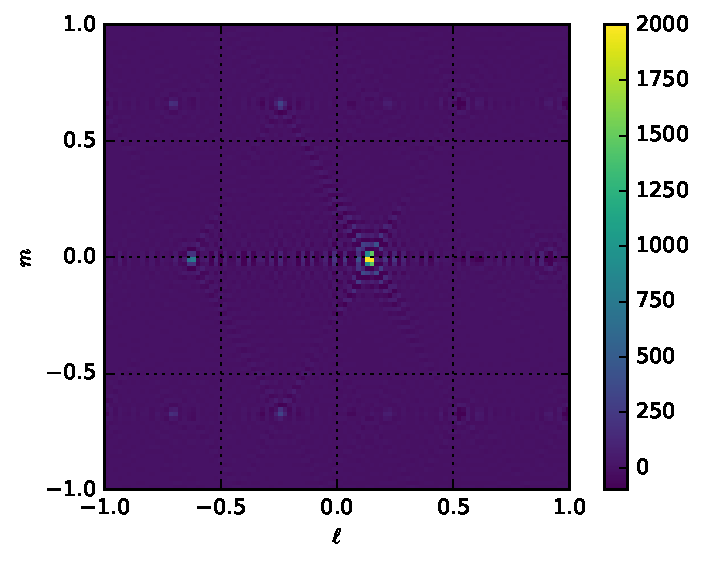
\includegraphics[width=.5\textwidth]{image_offZenith_217Ant_hex_dant_2_dantpos_3.pdf}
\caption{Image by a 217 antenna hexagonal array of a point source at $\ell=0.9,m=0$. The actual source is dwarfed by its side-lobe which is in the center of the primary beam.}
\label{fig:ImageHexDefault}
\end{figure}

In Fig.~\ref{fig:PowerSpectrumHexDefault} I show the power spectrum of gridded visibilities compared to those obtained with the delay transform techniques. The level of foreground isolation required to measure the 21\,cm signal is typically taken to be $10^{-5}$ so I plot the contour at which the foregrounds pass below $10^{-5}$ their peak value as a white-dashed contour. I plot the horizon wedge as a solid white line with a black-dashed line overlaid. We see that the foreground leakage from the gridded power spectrum vastly exceeds that in the delay-transform power spectrum. As is well known, redundant arrays are indeed abysmal for the imaging power-spectrum technique. 


\begin{figure*}
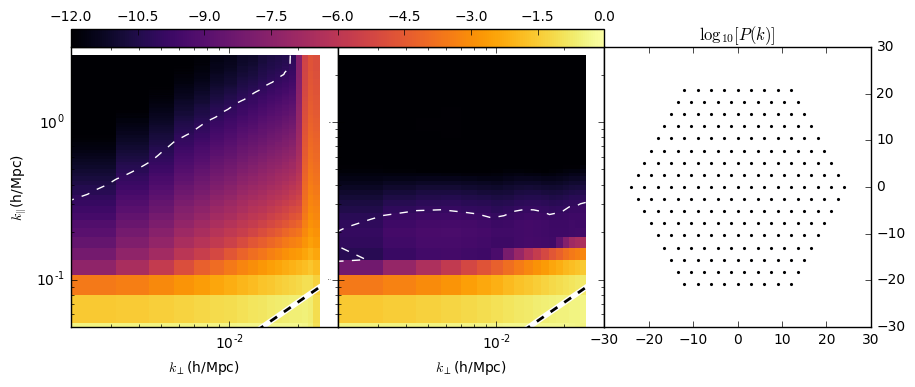
\includegraphics[width=\textwidth]{power_spectrum_hex_217_dAnt_2_dAntPos_3.png}
\caption{The cylindrical power spectrum for a 217 antenna hex array of 2\,m apertures spaced by 3\,m (Antenna positions are shown on the right). The horizon ``Wedge" is drawn as a thick white line with a dashed black line overlayed. We demarcate the contour at which the power spectrum of the sources drops below $10^{-5}$ its maximum as a white dashed line. This level of isolation is typically assumed to be what is required for a detection of the 21\,cm signal. Left: Power spectrum of gridded $uv$ data with sampling function divided out. Right: The delay-transform power spectrum of the hex. We see that a hex has very poor imaging power-spectrum capabilities.}
\label{fig:PowerSpectrumHexDefault}
\end{figure*}

\subsection{Results for a Perturbed Hexes}
Next, I perturb the locations of the hexagonally arranged antennas by $1/\sqrt{2}$ times their separations in a random direction. The resulting image at $150$\,MHz is shown in Fig.~\ref{fig:ImageHexPerturbedDefault}. We see that the side-lobes have been dramatically suppressed. 
\begin{figure}
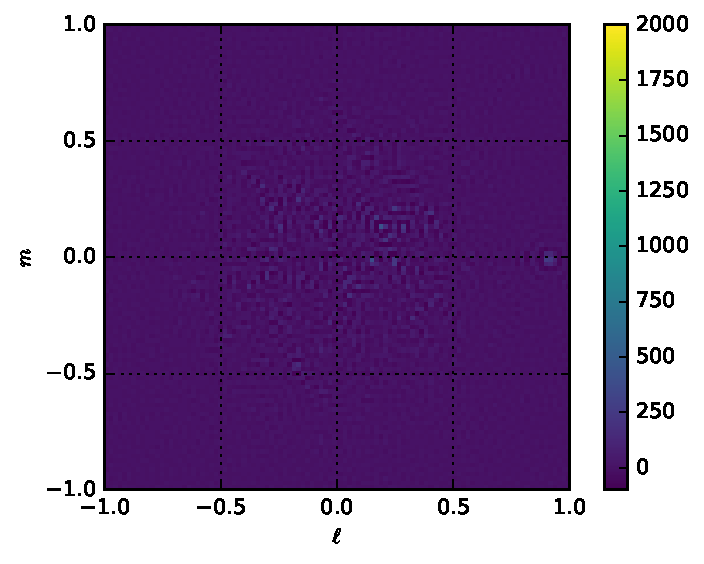
\includegraphics[width=.5\textwidth]{image_offZenith_217Ant_pHex_1config_dant_2_dantpos_3.pdf}
\caption{Image of a point source at $\ell=0.9$, $m=0$ by a 217 antenna hexagonal array of $2$\,m diameter apertures separated by $3$\,m with each position perturbed by $\sqrt{2}\times 3/2$\,m. The side-lobes have been significantly suppressed relative to the hexagonal case.}
\label{fig:ImageHexPerturbedDefault}
\end{figure}


\begin{figure*}
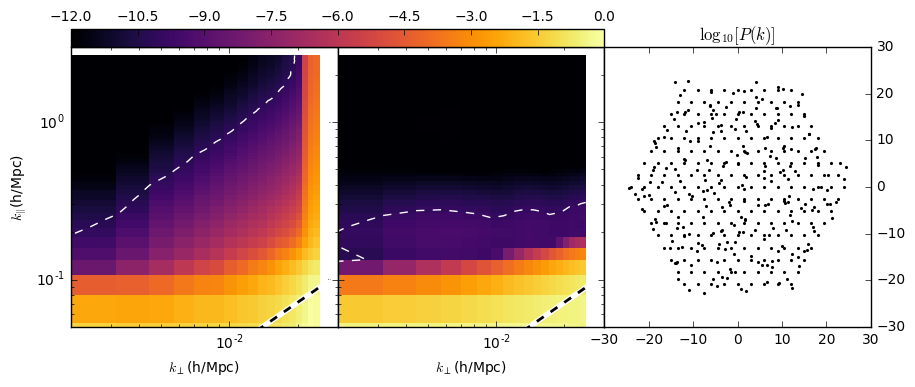
\includegraphics[width=\textwidth]{power_spectrum_hex_217_dAnt_2_dAntPos_3_perturbedHex_1config.png}
\caption{The cylindrical power spectrum for a 217 antenna hex array of 2\,m apertures spaced by 3\,m (Antenna positions are shown on the right). The horizon ``Wedge" is drawn as a thick white line with a dashed black line overlayed. We demarcate the contour at which the power spectrum of the sources drops below $10^{-5}$ its maximum as a white dashed line. This level of isolation is typically assumed to be what is required for a detection of the 21\,cm signal. Left: Power spectrum of gridded $uv$ data with sampling function divided out. Right: The delay-transform power spectrum of the hex. We see that significant improvements in the imaging power spectrum ar obtained. However, contamination still extends beyond what exists for the delay-transform wedge. }
\label{fig:PowerSpectrumPerturbedDefault}
\end{figure*}

In Fig.~\ref{fig:PowerSpectrumPerturbedDefault} I show the delay and imaging power spectrum of the perturbed Hex. We see that foreground leakage is dramatically improved but the region of k-space accessible is still significanlty smaller than that accessible through the delay-spectrum technique. 

\subsection{Co-adding Many Perturbed Configurations}
 Next I try co-adding 10 and 100 different independent perturbed configurations before dividing out the sampling function and Fourier transforming. The image of an imaged source at with 10 co-added configurations is shown in Fig.~\ref{fig:ImageHexPerturbedDefault_10Config}. We inspect a power spectrum comparision in Fig.~\ref{fig:PowerSpectrumPerturbedDefault_10Config}. While it is difficult to tell by simple inspection, some improvement has been achieved in the location of the $10^{-5}$ contour in the power spectrum (by $\approx 0.1 h$/Mpc). This convergence is alarmingly slow and I'm hesitant to say that I'm actually doing this right (dividing out the correct sampling function). I repeat the experiment for 100 random configurations with the power spectrum showin in Fig.~\ref{fig:PowerSpectrumPerturbedDefault_100Config}. To check that the gridded visibilities make sense, I show the gridded visibilities for various frequencies in Fig.~\ref{fig:VisPlot_100Config}.


\begin{figure}
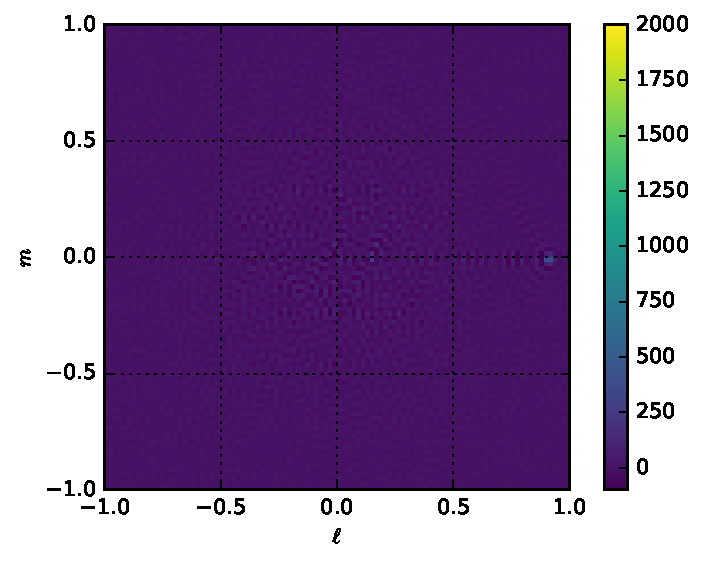
\includegraphics[width=.5\textwidth]{image_offZenith_217Ant_pHex_10config_dant_2_dantpos_3.pdf}
\caption{Image of a point source at $\ell=0.9$, $m=0$ by a 217 antenna hexagonal array of $2$\,m diameter apertures separated by $3$\,m with each position perturbed by $\sqrt{2}\times 3/2$\,m. Now the $uv$ distribution has been integrated over 10 random perturbations to the Hex. The side-lobes have been significantly suppressed relative to the hexagonal case.}
\label{fig:ImageHexPerturbedDefault_10Config}
\end{figure}

\begin{figure*}
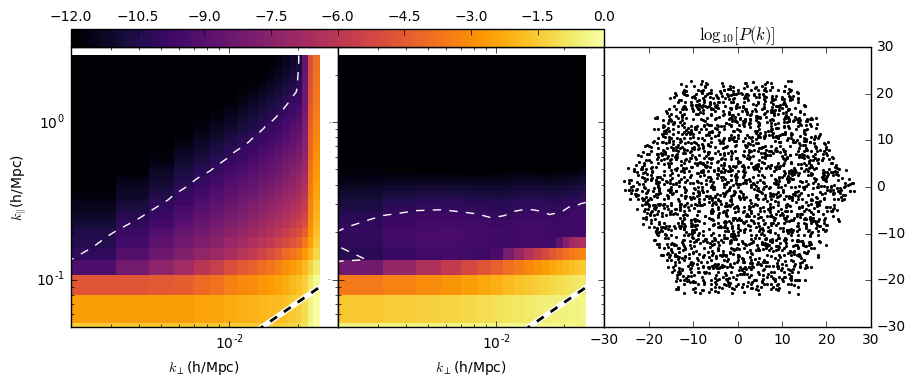
\includegraphics[width=\textwidth]{power_spectrum_hex_217_dAnt_2_dAntPos_3_perturbedHex_10config.png}
\caption{The cylindrical power spectrum for a 217 antenna hex array of 2\,m apertures spaced by 3\,m (Antenna positions are shown on the right). The antennas are perturbed in 10 different random configurations and the visibilities are co-added to the same $uv$ plane. The horizon ``Wedge" is drawn as a thick white line with a dashed black line overlayed. We demarcate the contour at which the power spectrum of the sources drops below $10^{-5}$ its maximum as a white dashed line. This level of isolation is typically assumed to be what is required for a detection of the 21\,cm signal. Left: Power spectrum of gridded $uv$ data with sampling function divided out. Middle: The delay-transform power spectrum of the hex. We see that significant improvements in the imaging power spectrum ar obtained. However, contamination still extends beyond what exists for the delay-transform wedge. Right: Co-added antenna positions.}
\label{fig:PowerSpectrumPerturbedDefault_10Config}
\end{figure*}

\begin{figure*}
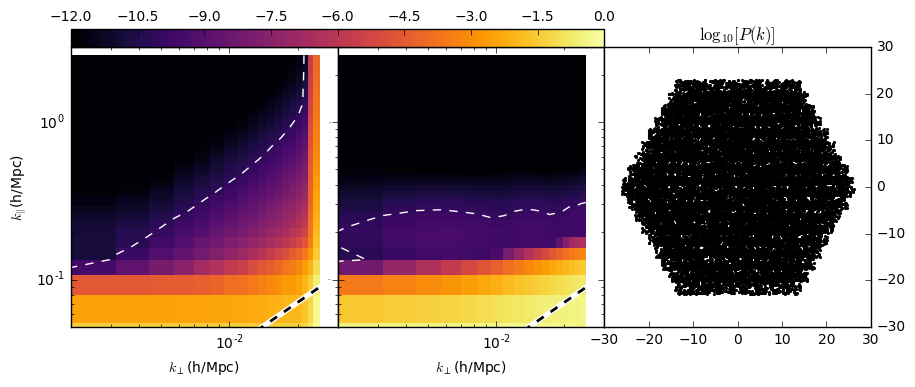
\includegraphics[width=\textwidth]{power_spectrum_hex_217_dAnt_2_dAntPos_3_perturbedHex_100config.png}
\caption{The cylindrical power spectrum for a 217 antenna hex array of 2\,m apertures spaced by 3\,m (Antenna positions are shown on the right). The antennas are perturbed in 100 different random configurations and the visibilities are co-added to the same $uv$ plane. The horizon ``Wedge" is drawn as a thick white line with a dashed black line overlayed. We demarcate the contour at which the power spectrum of the sources drops below $10^{-5}$ its maximum as a white dashed line. This level of isolation is typically assumed to be what is required for a detection of the 21\,cm signal. Left: Power spectrum of gridded $uv$ data with sampling function divided out. Middle: The delay-transform power spectrum of the hex. We see that significant improvements in the imaging power spectrum ar obtained. However, contamination still extends beyond what exists for the delay-transform wedge. Right: Co-added Antenna positions.}
\label{fig:PowerSpectrumPerturbedDefault_100Config}
\end{figure*}

%%%%%%%%%%%%%%%%%%%%%%%%%%%%%%%%%%%%%%%%%%%%%%%%%%

%%%%%%%%%%%%%%%%%%%% REFERENCES %%%%%%%%%%%%%%%%%%

% The best way to enter references is to use BibTeX:

\begin{figure*}
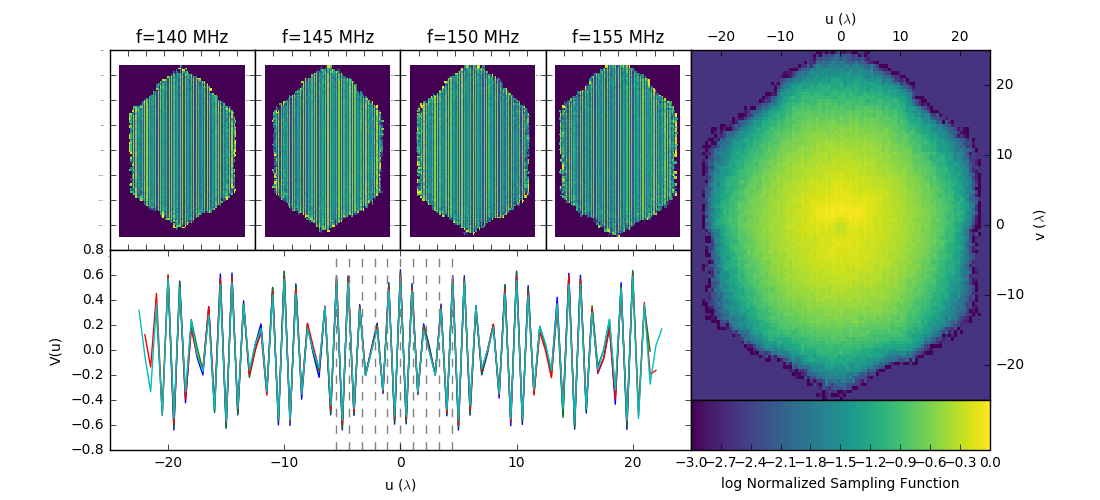
\includegraphics[width=\textwidth]{visPlot_217_perturbHex_100config_dAnt_2_dAntPos_3.png}
\caption{Top Left: the real component of the uniformly-weighted gridded visibilities for our off axis ($\ell=0.9$ source for several different frequency slices. Bottom: The average of the four slices along the $v-axis$ (where the sampling function was not zero). Right: The logarithm of the array sampling function, noramalized to unity. Some aliasing is visible on the bottom left plot due to the finite dish size. Vertical dashed lines indicate the expected locations of the fringe peaks.}
\label{fig:VisPlot_100Config}
\end{figure*}

\begin{figure*}
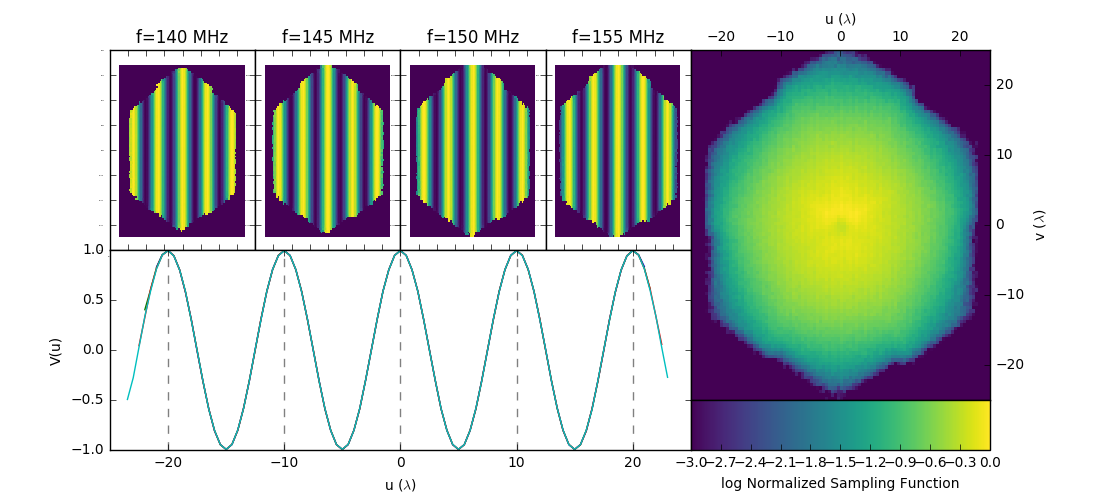
\includegraphics[width=\textwidth]{visPlot_offcenterleast_perturbHex_100config_dAnt_2_dAntPos_3.png}
\caption{Same as Fig.~\ref{fig:VisPlot_100Config} but for a source with $\ell=0.1$.}
\label{fig:VisPlot_100Config_nearZenith}
\end{figure*}

\begin{figure}
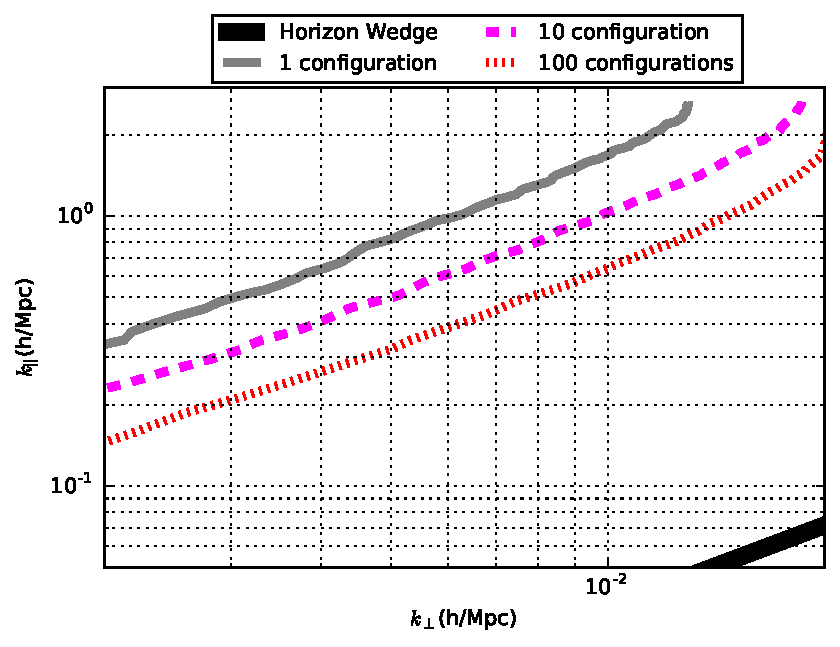
\includegraphics[width=.5\textwidth]{wedgeCompare_217_dAnt_2_dAntPos_3_offZenith_p9.pdf}
\caption{Lines in cylindrical k-space in which the foreground level goes below $10^{-5}$ its peak. Increasing the number of co-added integrations appears to monotonically improve the degree of foreground isolation but in all cases up to 100 co-added integrations, the contamination significantly exceeds the level. }
\label{fig:CompareContoursIntegrations}
\end{figure}


\begin{figure}
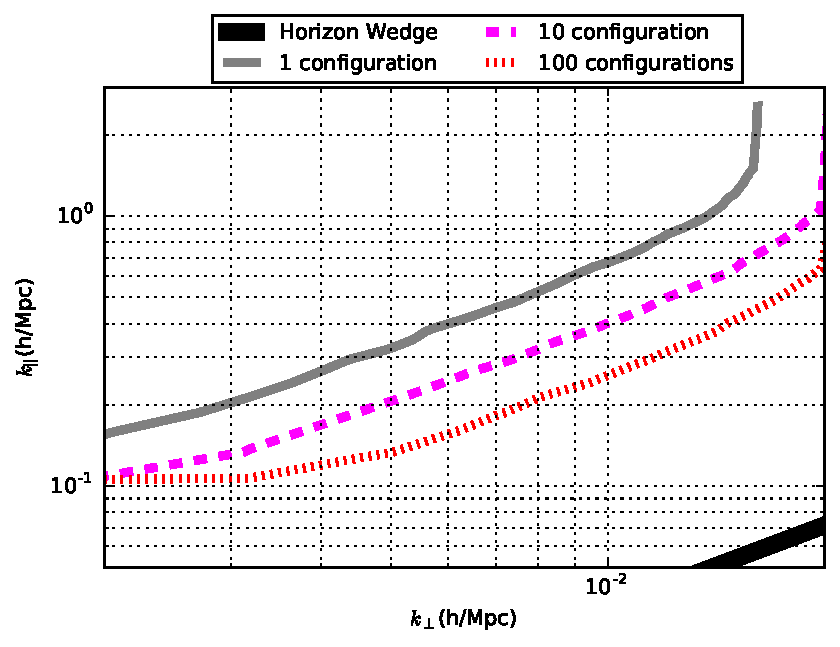
\includegraphics[width=.5\textwidth]{wedgeCompare_217_dAnt_2_dAntPos_3_offcenterleast_p9.pdf}
\caption{Same as Fig.~\ref{fig:CompareContoursIntegrations} but for a single source with $\ell=0.1$ instead of $\ell=0.9$. }
\label{fig:CompareContoursIntegrations_nearZenith}
\end{figure}


I perform the same exercise for sources at $\ell = \{0.1,0.25,0.5,0.0\}$. I show the resulting power spectra in Fig.~\ref{fig:PowerSpectrumPerturbDefault_DiffPositions}.


\begin{figure*}
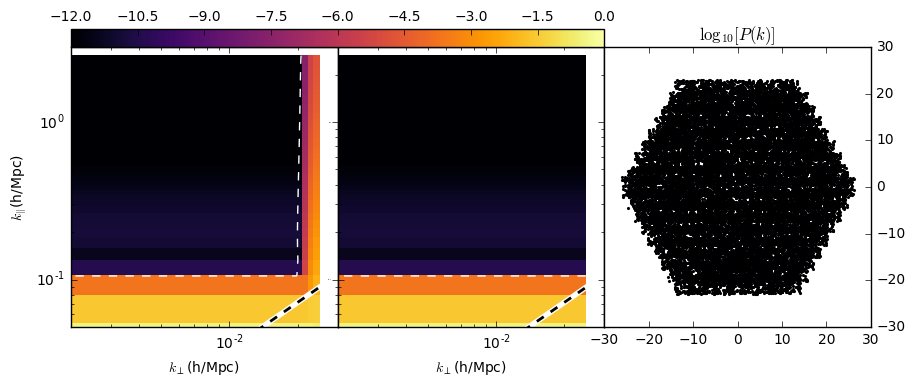
\includegraphics[width=\textwidth]{power_spectrum_zenith_hex_217_dAnt_2_dAntPos_3_perturbedHex_100config.png}
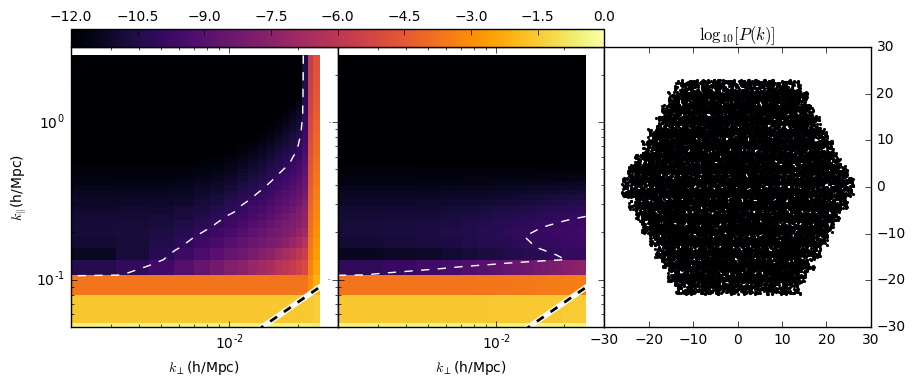
\includegraphics[width=\textwidth]{power_spectrum_offcenterleast_hex_217_dAnt_2_dAntPos_3_perturbedHex_100config.png}
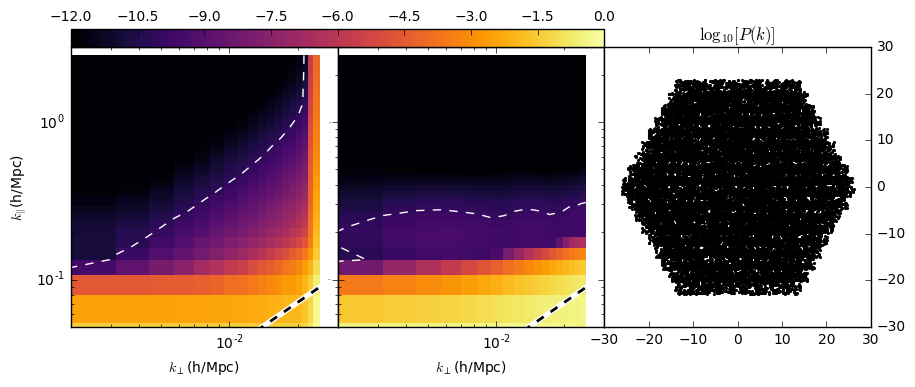
\includegraphics[width=\textwidth]{power_spectrum_hex_217_dAnt_2_dAntPos_3_perturbedHex_100config.png}
\caption{Power Spectra for 100 co-added antenna configurations with 2\,m apertures spaced 3\,m apart and perturbed $3 \times \sqrt{2}/2$\,m for sources at $\ell = 0$(top), $\ell=0.1$ (middle) and $\ell=0.9$ (bottom). We see that a zenith sourch in both the imaging and visibility power spectrum is centered at $k_\parallel=0$ with no leakage. A source that is only six degrees off zenith imposes significant leakage in the imaging power spectrum.}
\label{fig:PowerSpectrumPerturbDefault_DiffPositions}
\end{figure*}

The slow rate at which a single foregrounds contamination is mitigated through co-added integrations is somewhat discouraging. I will try looking at a filled aperture and than move to larger antennas with fewer elements (to reduce the primary beam width). One possibility is that large moveable antennas can be implemented in software by phased different sub-arrays over each night. 

\subsection{Multiple Sources}
\subsection{Filled Aperture Perturbed Hex}
\subsection{Large Antennas}

\bibliographystyle{mnras}
\bibliography{moveableAntenna} % if your bibtex file is called example.bib


% Alternatively you could enter them by hand, like this:
% This method is tedious and prone to error if you have lots of references
%\begin{thebibliography}{99}
%\bibitem[\protect\citeauthoryear{Author}{2012}]{Author2012}
%Author A.~N., 2013, Journal of Improbable Astronomy, 1, 1
%\bibitem[\protect\citeauthoryear{Others}{2013}]{Others2013}
%Others S., 2012, Journal of Interesting Stuff, 17, 198
%\end{thebibliography}

%%%%%%%%%%%%%%%%%%%%%%%%%%%%%%%%%%%%%%%%%%%%%%%%%%

%%%%%%%%%%%%%%%%% APPENDICES %%%%%%%%%%%%%%%%%%%%%

%\appendix

%\section{Some extra material}

%If you want to present additional material which would interrupt the flow of the main paper,
%it can be placed in an Appendix which appears after the list of references.

%%%%%%%%%%%%%%%%%%%%%%%%%%%%%%%%%%%%%%%%%%%%%%%%%%


% Don't change these lines
\bsp	% typesetting comment
\label{lastpage}
\end{document}

% End of mnras_template.tex